\documentclass{ctacn}
\usepackage{hhline}
\usepackage{hyperref}
\usepackage{enumitem}

\newcommand{\zhnauthora}{张航宁}
\newcommand{\zhnauthorb}{吴嘉伟}
\newcommand{\zhnauthorc}{潘倩}
\newcommand{\zhnauthord}{鹿思淇}
\newcommand{\zhnauthore}{胡泽辰}
\newcommand{\zhncntitle}{小推力地火转移轨道设计与优化}
\newcommand{\zhnentitle}{(Undetermined)}
\newcommand{\zhncnabstract}{
    任务目标:固定转移时间的燃耗最优转移。
    输出结果:转移轨道、推力曲线、开关函数。
    提交形式:pdf报告、latex程序压缩包、c++程序压缩包、exe仿真展示软件。}
\newcommand{\zhncnkeyword}{小推力;地火转移轨道}
\newcommand{\zhnenabstract}{None.}
\newcommand{\zhnenkeyword}{None}

\begin{document}

%%%%%%%
\cndoi{}
\doi{\zihao{-5}10.13195/j.kzyjc.2019.0000}
\paperdate{2022-xx-xx}{2022-xx-xx}%接收日期,修回日期
\osid{}
\setcounter{page}{1}

%%%%%%%%%%
%%%%%%%输入页眉显示的题目
%%%%%%%%%%%%
\runheading{\zhnauthora~等: \zhncntitle}%页眉设置,填写第一作者及论文题目
\xiangmujijin{}%项目基金  为空会自动取消显示
\authorcor{E-mail: yz37zhn@163.com.}%通讯作者邮箱,新投稿不修改
\cntitle{\zhncntitle}  % 输入中文标题
\entitle{\zhnentitle}


%                  新投稿不要修改下面的姓名及单位
%%%中文作者和单位,\dag代表通信作者,“作者一”代表3个字的名,“作者”代表2个字的名
\cnauthor{\zhnauthora\makebox{$^{1\dag}$},~~\zhnauthorb\makebox{$^{2}$},~~\zhnauthorc\makebox{$^{2}$},~~\zhnauthord\makebox{$^{2}$},~~\zhnauthore\makebox{$^{2}$}}  %新投稿不修改
{(1.北京控制工程研究所,北京100094;2. 北京理工大学,北京100081)}  %%省会城市无需加省%%新投稿不要修改

%%%中文摘要
\cnabstract{\zhncnabstract}

%%%中文关键词
\cnkeyword{\zhncnkeyword}

%%%分类号、标识码
\clc{V}  % 中文分类号,请作者自行查找并填写
\wenxianbiaoshi{A}  % 文献标志码

\citation{}

%%%%%%%              新投稿不要修改下面的英文名及单位
\enauthor{Hangning Zhang\makebox{$^{1\dag}$}}{
(1. China Academy of Space Technology,Beijing~100094,China)}
\enabstract{\zhnenabstract}
\enkeyword{\zhnenkeyword}
\maketitle

\begin{multicols}{2}

%%%%%%%%%%%%%%%%%%%%%%%%%%%%%%%%%%%%%%%%%%%%%%%%%%%%%%%%%%%%%%%%
% 正文
%%%%%%%%%%%%%%%%%%%%%%%%%%%%%%%%%%%%%%%%%%%%%%%%%%%%%%%%%%%%%%%%
\section{引\quad 言}行星际转移轨道优化设计是轨道动力学与控制研究中的热点问题。在连续推力作用下,探测器的轨道动力学非线性强,可行轨道解空间非常复杂,如何在复杂约束下寻找最优的转移轨道是研究的难点,其本质是一个强非线性连续最优控制问题。目前,求解该问题的方法主要分为直接法和间接法两类,这两类方法的主要区别是对控制量的参数化方式不同。

%%%%%%%%%%%%%%%%%%%%%%%%%%%%%%%%%%%%%%%%%%%%%%%%%%%%%%%%%%%%%%%%
% Form
%%%%%%%%%%%%%%%%%%%%%%%%%%%%%%%%%%%%%%%%%%%%%%%%%%%%%%%%%%%%%%%%
\section{基本公式}
下面推列举一些需要用到的公式定理。

% ////////////////////////////////////////
\subsection{改进春分点轨道根数}
改进的春分点轨道与开普勒轨道根数之间的转换关系定义如下\cite{mxubo2016}:
\begin{align}
    \begin{aligned}
        p =& a\left(1-e^{2}\right) \\
        f =& e \cos (\omega+\Omega) \\
        g =& e \sin (\omega+\Omega) \\
        h =& \tan (i / 2) \cos \Omega \\
        k =& \tan (i / 2) \sin \Omega \\
        L =& \Omega+\omega+\theta
    \end{aligned} \label{eqFormEquinoctial1}
\end{align}
\begin{align}
    \begin{aligned}
        a =& \frac{p}{1-f^{2}-g^{2}} \\
        e =& \sqrt{f^{2}+g^{2}} \\
        i =& 2 \arctan \sqrt{h^{2}+k^{2}} \\
        \Omega =& \arctan \left(\frac{k}{h}\right) \\
        \omega =& \arctan \left(\frac{g}{f}\right)-\arctan \left(\frac{k}{h}\right) \\
        \theta =& L-\arctan \left(\frac{g}{f}\right)
    \end{aligned} \label{eqFormEquinoctial2}
\end{align}
式\eqref{eqFormEquinoctial1}\eqref{eqFormEquinoctial2}分别表示
开普勒转改进春分点和改进春分点转开普勒轨道根数。

% ////////////////////////////////////////////////////////////////
\subsection{轨道六根数和位置速度向量}
给定一个轨道物体的轨道六要素后,
即可计算出该物体相对于中心引力源的位置和速度向量,
换算关系为
\begin{align}
    R =& \left[\begin{matrix}
        c_\Omega c_\omega-s_\Omega c_i s_\omega & -c_\Omega s_\omega-s_\Omega c_i c_\omega & s_\Omega s_i \\
        s_\Omega c_\omega+c_\Omega c_i s_\omega & -s_\Omega s_\omega+c_\Omega c_i c_\omega & -c_\Omega s_i \\
        s_i s_\omega & s_i c_\omega & c_i
    \end{matrix}\right] \notag\\
    \vec{r} =& R\left[\begin{matrix}
        \frac{a(1-e^2)}{1+e\cos\theta}\cos\theta \\ \frac{a(1-e^2)}{1+e\cos\theta}\sin\theta \\ 0
    \end{matrix}\right] \notag\\
    \vec{v} =& R\left[\begin{matrix}
        -\sqrt{\frac{\mu}{a(1-e^2)}}\sin\theta \\ \sqrt{\frac{\mu}{a(1-e^2)}}(e+\cos\theta) \\ 0
    \end{matrix}\right] \label{eqFormEle2RV}
\end{align}
其中$\theta$为真近点角。
若已知初始时刻的轨道六要素,
求给定时刻的位置速度向量的步骤为
\begin{enumerate}[label={(\arabic*)}]\setlength{\itemsep}{-5pt}
    \item 根据轨道六要素求出平均角速度和初始平近点角;
    \item 根据初始平近点角、平均角速度、给定时刻求出给定时刻的平近点角;
    \item 由平近点角计算真近点角;
    \item 将给定时刻的真近点角代入式\eqref{eqFormEle2RV}计算位置速度向量;
\end{enumerate}
上述步骤需要平近点角和真近点角之间的换算。
由真近点角计算平近点角公式为
\begin{align*}
    E =& 2\arctan\left(\sqrt{\frac{1-e}{1+e}}\tan\frac{\theta}{2}\right) \\
    M =& E - e\sin{E}
\end{align*}
其中$E$为偏近点角,且与真近点角位于同一象限。
由平近点角$M$计算真近点角$\theta$没有解析解,
需要使用泰勒展开的方法,
具体公式如下\cite{msmart1977}
\begin{align*}
    \theta =& M+\left(2e-\frac{1}{4}e^3\right)\sin{M}
    + {\frac{5}{4}}e^2\sin{2M} \\
    &+ {\frac{13}{12}}e^3\sin{3M}+O(e^4)
\end{align*}


%%%%%%%%%%%%%%%%%%%%%%%%%%%%%%%%%%%%%%%%%%%%%%%%%%%%%%%%%%%%%%%%
% Real
%%%%%%%%%%%%%%%%%%%%%%%%%%%%%%%%%%%%%%%%%%%%%%%%%%%%%%%%%%%%%%%%
\section{无量纲处理}
宇宙中各天体的自转或公转周期通常以天甚至以年计算,
且轨道速度快,空间尺度大。
如果按照实际参数进行仿真,
则仿真的计算量太大而无法实时计算。
为了能够在仿真时直观地实时展示仿真结果,
需要对一些公式的单位进行换算。

万有引力公式
\begin{equation*}
    \frac{\text{d}^2\vec{r}}{\text{d}t^2}=-\frac{\mu}{r^3}\vec{r}
\end{equation*}
中,$r$的单位是km,$t$的单位是s。
因为实际的尺度太大,一个天文单位达到了$10^8$数量级,
为了便于仿真,
需要将实际尺度中的时间和距离变换到一个合适的时空坐标系下。
首先列举一些名词解释。
\textbf{实际时间}指宇宙尺度上的实际时间;
\textbf{无单位求解器时间}指微分方程求解器中自变量的值,
没有单位,简称求解器时间,
对应的求解器速度和求解器距离也都没有单位;
\textbf{仿真展示软件消耗时间}:例如仿真展示软件运行1秒对应实际时间的1000秒,
此处的1秒指的是是仿真展示软件消耗时间,简称展示时间。

举例说明,
求解器时间的1单位时间等于实际时间的$10^4$秒,
1单位距离等于实际距离$10^6$km,即在求解器中,
\begin{equation}
    \bar{t}=10^{-4}t,\ \bar{r}=10^{-6}r \label{eqRealConvert}
\end{equation}
其中$t$和$r$分别为以秒和千米为单位的实际时间和实际距离,
而$\bar{t}$和$\bar{r}$分别表示求解器时间和求解器距离。
1个天文单位为$r=1.5\times10^8$km,
则求解器中的1个天文单位为$\bar{r}=150$。
然后可以计算出实际时间/速度/距离
和求解器时间/速度/距离之间的一些换算关系
\begin{align*}
&\bar{v} = \frac{\text{d}\bar{r}}{\text{d}\bar{t}}
 = \frac{10^{-6}\text{d}r}{10^{-4}\text{d}t} = 10^{-2}v \\
&\bar{a} = \frac{\text{d}}{\text{d}\bar{t}}\frac{\text{d}\bar{r}}{\text{d}\bar{t}}
 = 10^2\frac{\text{d}^2r}{\text{d}t^2} = 10^2a \\
&\bar{\mu}\left[\frac{(10^{-6}\text{km})^3}{(10^{-4}\text{s})^2}\right]
 = 10^{-10}\mu\left[\frac{\text{km}^3}{\text{s}^2}\right] \\
&-\frac{\bar{\mu}}{\bar{r}^2} = -10^2\frac{\mu}{r^2}
 = 10^2\frac{\text{d}^2r}{\text{d}t^2} = \bar{a}
\end{align*}
其中引力常数$\mu$的单位中包含时间/距离量纲,
因此也需要换算。
可以验证,实际中的微分方程
$$a=-\frac{\mu}{r^2}$$
变换到求解器中仍然为
$$\bar{a}=-\frac{\bar{\mu}}{\bar{r}^2}$$

下面在换算公式\eqref{eqRealConvert}的基础上引入仿真展示软件消耗时间。
若仿真步长设置为0.01求解器时间,仿真展示软件每帧仿真10步,
则换算到实际时间上的步长为100秒,每帧代表1000秒,
按60帧计算,则展示时间1秒等于实际时间$6\times10^4$秒,
地球的轨道速度按30km/s算则展示时间1秒内地球走过$1.8\times10^6$km,
换算回仿真中则走过1.8展示距离。
换一种方法计算,
地球的求解器速度是$\bar{v}=10^{-2}\times30=0.3$,
仿真展示软件每1秒仿真:
60帧$\times$10步/帧$\times$0.01单位时间/步=6个时间单位,
也可以得到展示时间1秒内地球走过1.8展示距离。
在式\eqref{eqRealConvert}的设定下,
仿真展示软件每帧仿真1步与10步对应的地球自转周期分别约为$14.4$和$1.44$秒,
分别可用于展示低轨卫星和地球同步卫星的动态运行结果。

与实时仿真不同的是实际中广泛使用的非实时仿真,
也就是在一次仿真结束后展示静态仿真结果。
此时虽然不需要考虑展示时间/速度/距离,
但求解器时间/速度/距离仍然需要考虑。

单位换算在显著加快仿真速度的同时,
微分方程数值求解的精度也会受到影响。
已知四阶龙格库塔法的局部截断误差为$O(h^5$)\cite{mqingyang2019},
取无量纲步长为$h_0=10^{-3}$,
对微分方程
\[\frac{\text{d}\bar{r}}{\text{d}\bar{t}}=\bar{v}\]
局部截断误差为$\Delta\bar{r}=Ch_0^5=10^{-15}C$,
换算回真实值得到$\Delta r=10^6\Delta\bar{r}=10^{-9}C$,
同理可得
$\Delta v=10^2\Delta\bar{v}=10^{-13}C$,
$\Delta a=10^{-2}\Delta\bar{a}=10^{-17}C$。
以$r$为例,
换算单位前仿真10秒的累积误差为
\[e_1=10^4C\times 10^{-15}=10^{-11}C\]
换算单位后,时间单位换算成万秒,
仍取无量纲步长$h_0=10^{-3}$,
即实际步长为$h_2=10^{-3}$万秒,
仿真10秒就是1个步长,累积误差等于局部截断误差
\[e_2=10^{-9}C\]
若不换算单位而只是改变步长,
取步长$h_3=1$秒,
尽管实际上$h_3=10h_2$,
但仿真10秒的累积误差高达
\[e_3=10C\times 1^5=10C\]
因此在不同的仿真中,
在数值求解的仿真步长不变的前提下,
使用单位换算的方法可以显著提高仿真速度,
同时也能保证仿真精度不会显著下降,
对于一些高阶导量甚至提高了仿真精度。
(对这一现象我不是很理解)

%%%%%%%%%%%%%%%%%%%%%%%%%%%%%%%%%%%%%%%%%%%%%%%%%%%%%%%%%%%%%%%%
% Model
%%%%%%%%%%%%%%%%%%%%%%%%%%%%%%%%%%%%%%%%%%%%%%%%%%%%%%%%%%%%%%%%
\section{算法描述}
本文使用差分进化算法\cite{jqingfeng2017}求解转移轨道。
一般使用参数优化的方法是将推力离散化,
然后每个离散点的推力值算作一个参数,
优化每个离散点的推力值使得转移轨道的某些参数最优。
这样待优化的参数特别多\cite{dchengxing2011},
并且如果发动机工作时间不固定,
那么待优化的参数个数也就不固定,
而一般的启发式优化算法都假设了不同个体(不同的解)的参数个数相等。
另外由于推力一般连续变化且变化幅度不大,
但启发式算法一般也都假设各个参数之间独立,
也就是说推力问题中相邻的离散点的值有一定的约束,
但启发式算法解决带约束的问题比较吃力。
不知道有没有启发式算法解决约束问题较好的例子。

为此,文献\cite{jbradley2005}提出了将发动机推力变化曲线用三次多项式(cubic polynomials)拟合的方法,
在出发点和到达点附近分别使用了一个三次多项式来拟合发动机的推力方向。
这一方法既解决了参数约束的问题也解决了参数不固定的问题,
更极大减小了参数数量,
但作者认为这种方法达不到最优解。
本文使用这种方法,
另外考虑地球轨道和火星轨道不共面的情况,
在推力方向中加入了俯仰角,
因此多了两个三次多项式。

文献\cite{jbradley2005}也提出了将发动机工作的起止时间也作为待优化参数的思想,
但没有提到如何处理超过参数变化范围的情况,
比如发动机工作时间不可能是负数。
就算在初始化时只生成正数解,
但交叉和变异操作也可能会生成负数。
另外发动机工作时间也不能太长。
考虑到探测器质量一直在下降,
总的轨道转移时间为$22464e3$秒,
因此将加速和减速阶段的发动机工作时间分别限制在
$12500e3$秒和$7500e3$以内。
使用非线性公式、
\[T=k\arctan{x}^2\]
实施限制,
其中$k$值在加速和减速阶段分别为$\frac{25000}{\pi}$和$\frac{15000}{\pi}$,
$x$为服从标准正态分布的随机数,
用于启发式算法的初始化。

前一节中提到将实际时间加快$10^4$倍,
求解器一个步长对应10秒的实际时间,
则转移轨道全程总共约需要计算$2e6$个步长,
在个人电脑上计算完全程耗时约50秒。
为了能够使用启发式算法,
需要进一步加快速度。
保持距离换算关系不变,
将时间换算关系改为$\bar{t}=10^{-6}t$,
则

%%%%%%%%%%%%%%%%%%%%%%%%%%%%%%%%%%%%%%%%%%%%%%%%%%%%%%%%%%%%%%%%
% Sim
%%%%%%%%%%%%%%%%%%%%%%%%%%%%%%%%%%%%%%%%%%%%%%%%%%%%%%%%%%%%%%%%
\section{仿真}
本文使用基于C++的仿真器\cite{olzhn2021}进行仿真。

% ////////////////////////////////////////
\subsection{给定参数计算}
根据给定出发点和到达点的改进春分点轨道根数,
计算可得开普勒轨道根数为
\begin{center}\begin{tabular}{lll}
    \toprule
    名称 & 地球 & 火星 \\
    \midrule
    半长轴    a & $ 1.000840$ & $ 1.523677$ \\
    偏心率    e & $ 0.016507$ & $ 0.093435$ \\
    轨道倾角  i & $ 0.000021$ & $ 0.032276$ \\
    升交点赤经Ω & $ 0.030896$ & $ 0.864609$ \\
    近地点幅角ω & $-1.422358$ & $-1.281742$ \\
    真近点角    & $ 3.824526$ & $ 6.182348$ \\
    $\mu$值     & $398601   $ & $42808    $ \\
    \bottomrule
\end{tabular}\end{center}
可算出以速度为单位的比冲为$I_{sp}=19600$m/s,
也就是说保持发动机推力$F=1$N时,
燃料消耗速度为$d_m=1/19600$千克/秒,
限制发动机工作时间不超过总质量的40\%,
即$T_f=19600*400=7.84\times10^6$秒,约90天。
为统一单位,将长度单位全部换算成km,
则推力为$F=10^{-3}$kN。

% ////////////////////////////////////////
\subsection{建模}
假设探测器在转移轨道上不受地球和火星引力影响。
考虑燃料消耗的火星探测器动力学方程为
\begin{align}
    &\ddot{\vec{r}} = -\frac{\mu_s}{||\vec{r}||^3}\vec{r}
    + \frac{10^{-3}}{m(t)}\epsilon(t)
    \left[\begin{matrix}
        \cos\phi\cos\theta \\ \cos\phi\sin\theta \\ \sin\phi
    \end{matrix}\right] \label{eqSimAcc} \\
    &\dot{m}(t) = -\frac{1}{19600}\epsilon(t) \notag
\end{align}
其中
$\phi$和$\theta$分别为发动机推力向量的俯仰角和方位角,
$\epsilon(t)=0$或$1$表示发动机开机或关机。
建立探测器被控对象模型的模块框图如图\ref{figSimPlant}所示。
\begin{center}
	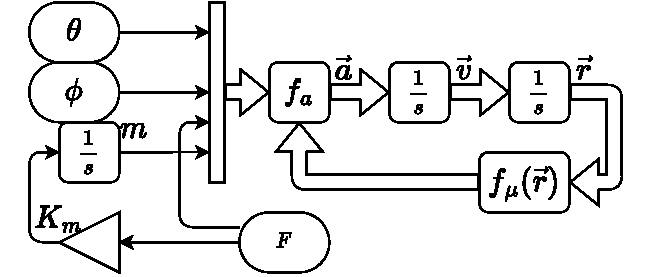
\includegraphics[scale=0.8]{plant.pdf}  \\
	\figcaption{火星探测器被控对象模型的模块框图}\label{figSimPlant}
\end{center}
其中$K_m=-\frac{\bar{d}_m}{\bar{F}}$。
$K_m\cdot F$为燃料消耗速度,作为质量积分器的输入。
有三个输入模块,分别为
发动机方位角$\theta$、俯仰角$\phi$、推力大小$F$,
这三个输入是待优化的时间函数。
函数模块$f_\mu(\vec{r})$计算引力加速度的系数
\[f_\mu(\vec{r})=-\frac{\mu_s}{||\vec{r}||^3}\]
输入为位置向量,输出为标量。
函数模块$f_a$计算加速度向量,即式\eqref{eqSimAcc},
输入为$\theta$、$\phi$、$F$、$m$这4个标量,输出为加速度向量。

% ////////////////////////////////////////
\subsection{仿真调试}
为了验证建模与仿真结果正确,
将部分调试步骤和中间结果记录如下。

\noindent\textbf{绘制轨道}\par
为验证出发点与到达点结果正确,
分别从出发点与到达点开始绘制半个公转周期轨道作为参考,如图\ref{figSimDebug1}所示。
\begin{center}
	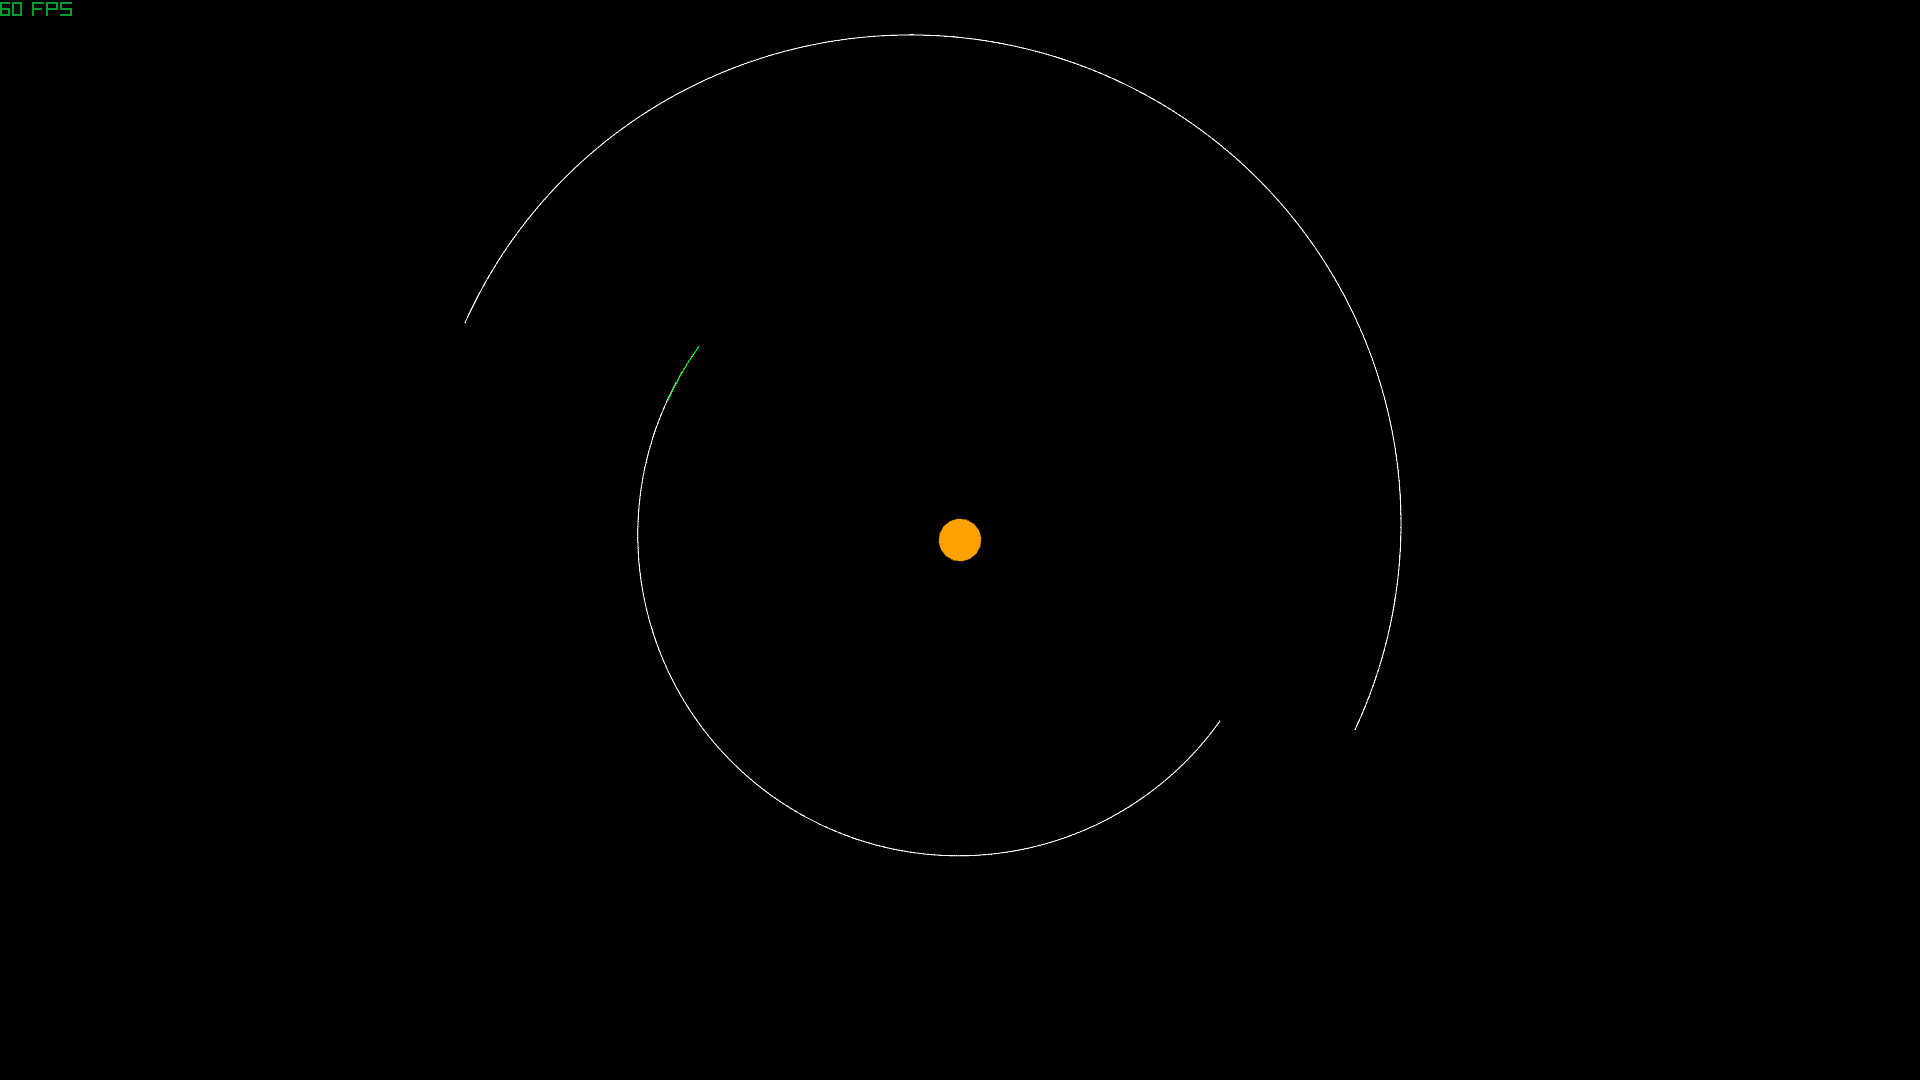
\includegraphics[scale=0.2]{simdebug1.png}  \\
	\figcaption{地球和火星的半个公转周期轨道俯视图}\label{figSimDebug1}
\end{center}
地球和火星的公转周期分别按365天和687天计算,
半个公转周期分别约为$1577$和$2968$仿真器秒。
1仿真器秒等于$1000$仿真步长,
1仿真步长等于实际时间10秒。
仿真器坐标下的出发点位置和速度向量分别为
\[[\begin{matrix}
    -113.102 & 101.033 & 0.00219
\end{matrix}]^\text{T}\]
\[[\begin{matrix}
    -0.19353 & -0.22118 & -4.517067e-06
\end{matrix}]^\text{T}\]
结果基本正确。

\noindent\textbf{燃料消耗}\par
仿真$10^5$个步长后,
仿真得剩余总质量为$948.98$kg。
$10^5$个步长对应$10^6$秒,
计算得燃料消耗$10^6\times\frac{1}{19600}=51.02$kg,
结果正确。
图\ref{figSimDebug1}中的绿色轨迹为
发动机推力俯仰角为0,方位角为$\theta-1.57$时持续工作$10^5$个步长的结果。

% ////////////////////////////////////////
\subsection{结果展示}
使用差分进化算法优化结果如图\ref{figSimAns1}所示。
两图分别为接近俯视图和接近侧视图。
对应的损失函数为$e=352.849$,
总质量剩余$634.133$kg。
\begin{center}
	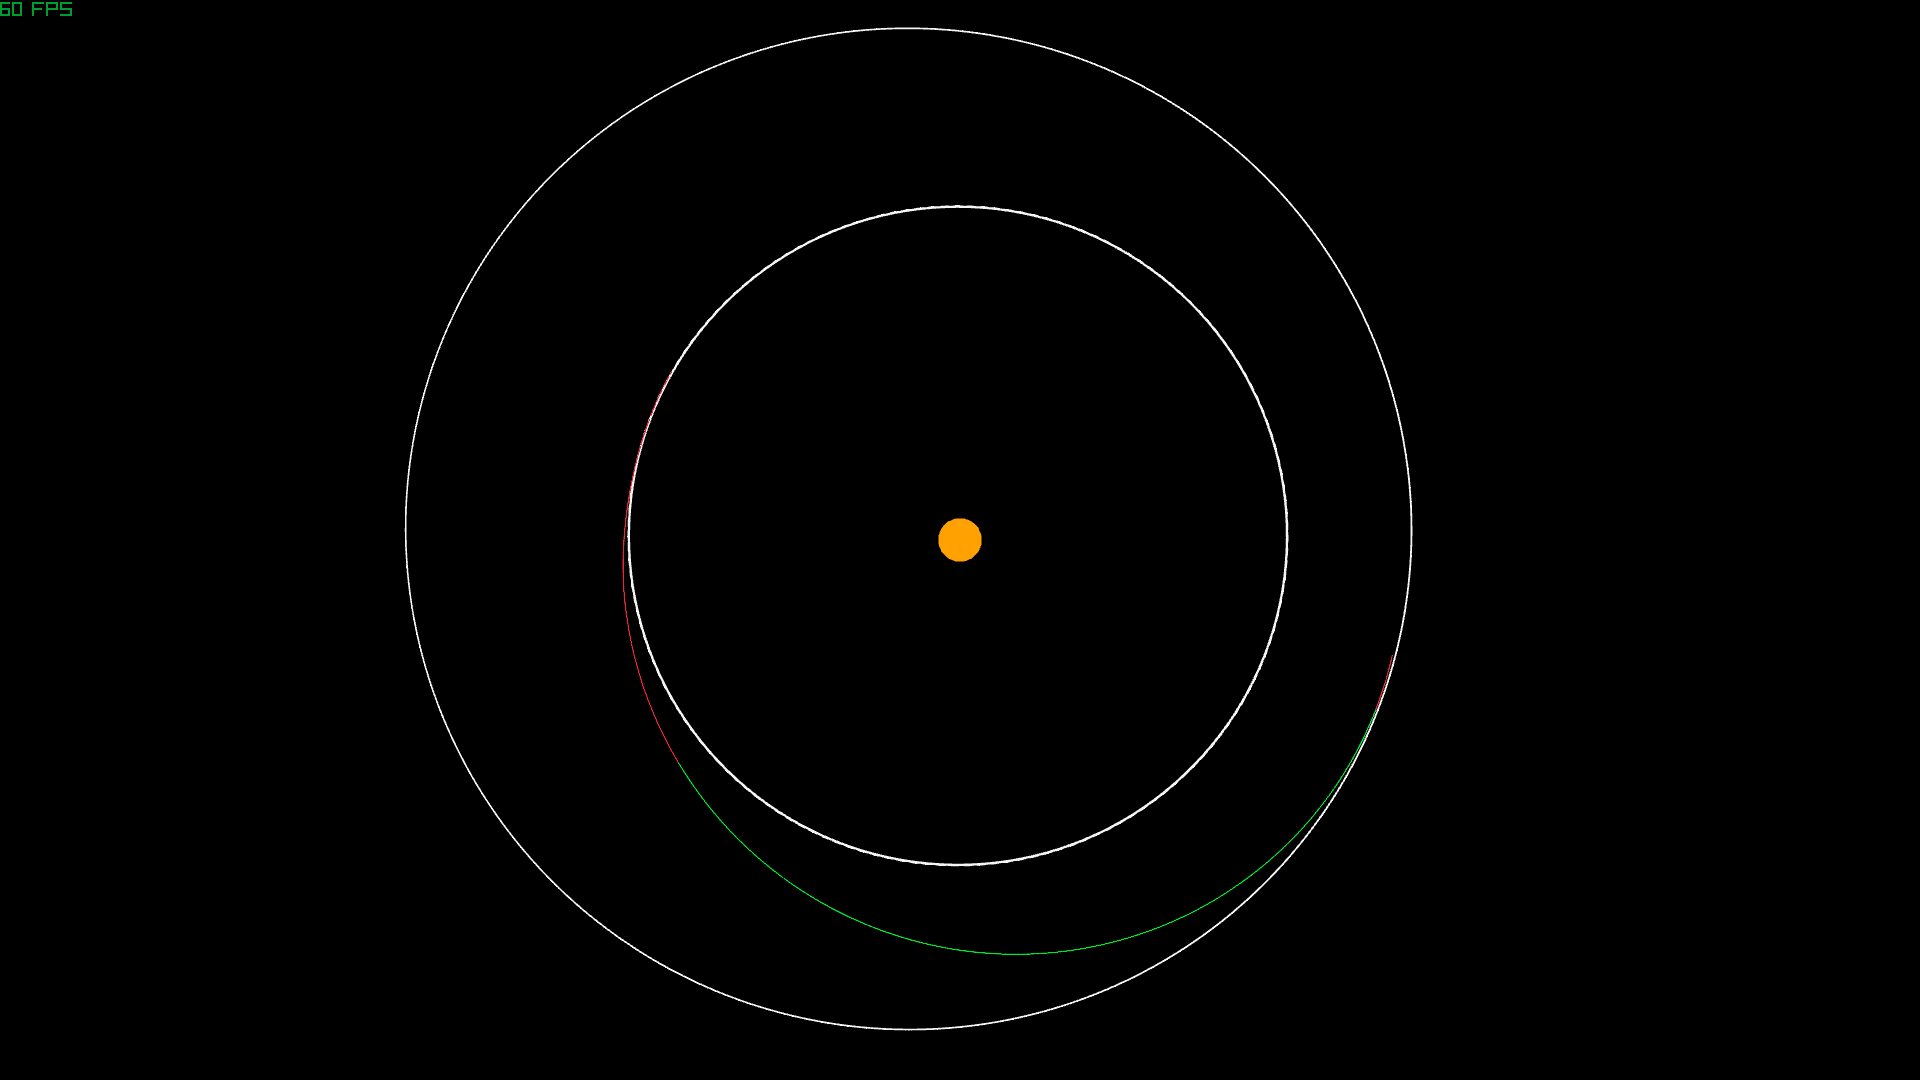
\includegraphics[scale=0.2]{simans1.png}  \\
	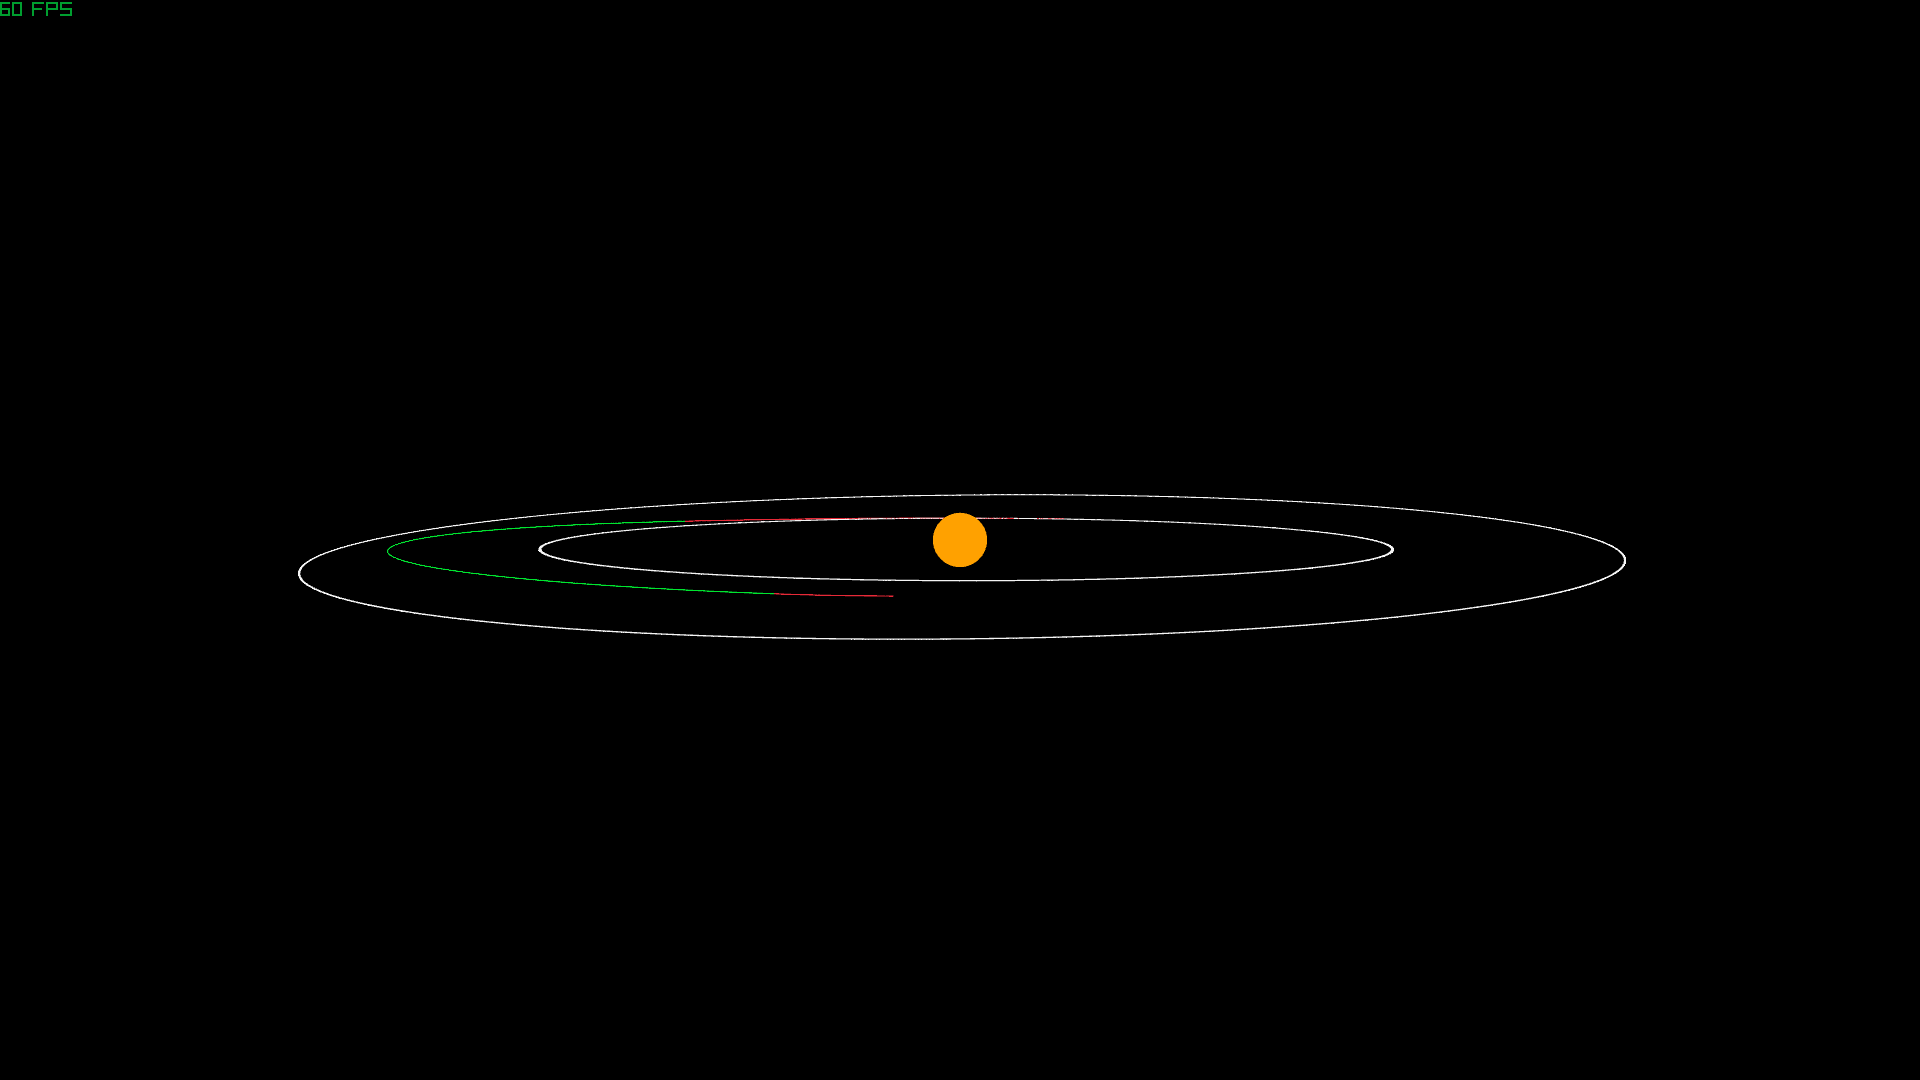
\includegraphics[scale=0.2]{simans2.png}  \\
	\figcaption{差分进化算法优化结果}\label{figSimAns1}
\end{center}
因为优化算法使用的时间单位是$10^6$秒,
是图\ref{figSimDebug1}中的100倍,
所以图\ref{figSimAns1}中地球和火星的轨道画了50圈。

使用模式搜索法优化结果如图\ref{figSimAns2}所示。
此时将损失函数中燃料消耗的比重由$10^{-2}$改为$10^{-3}$,
对应的优化后的损失函数为$e=78.870$,
总质量剩余$579.796$kg。
\begin{center}
	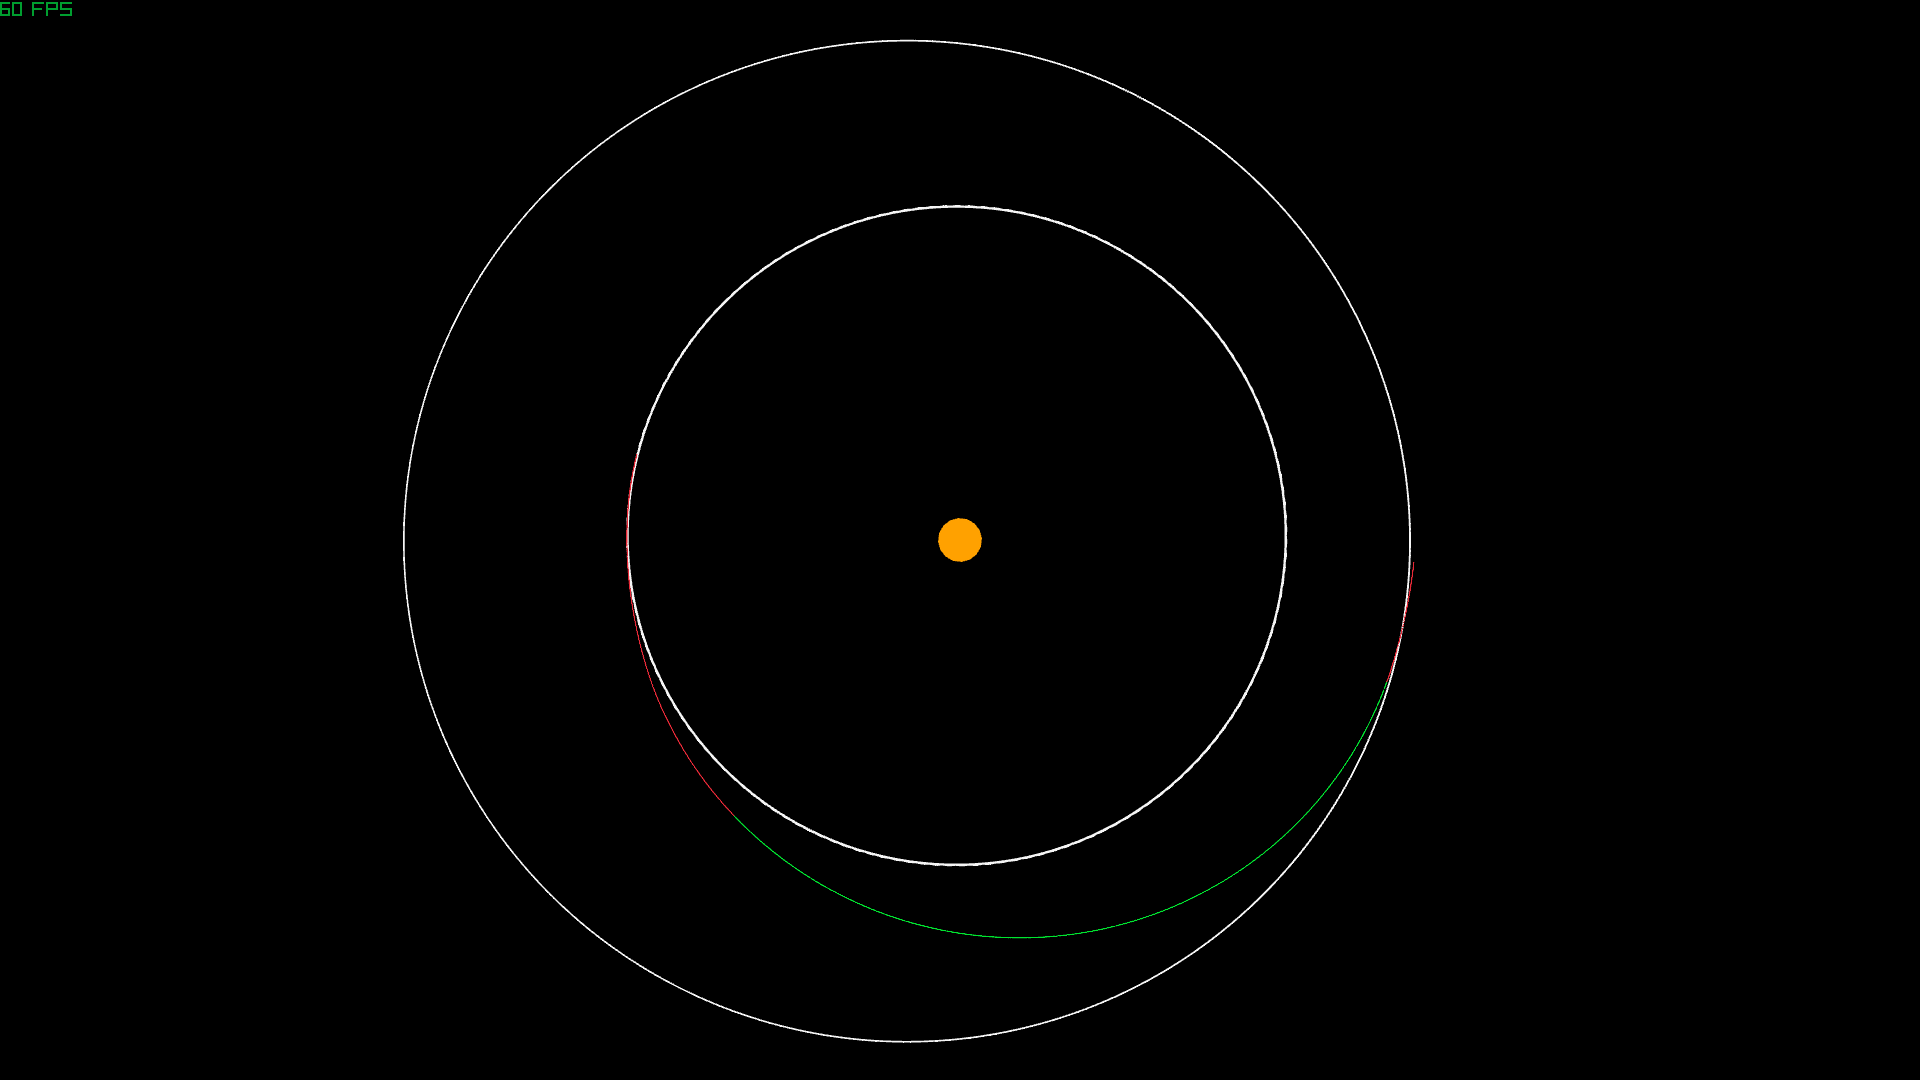
\includegraphics[scale=0.2]{simans3.png}  \\
	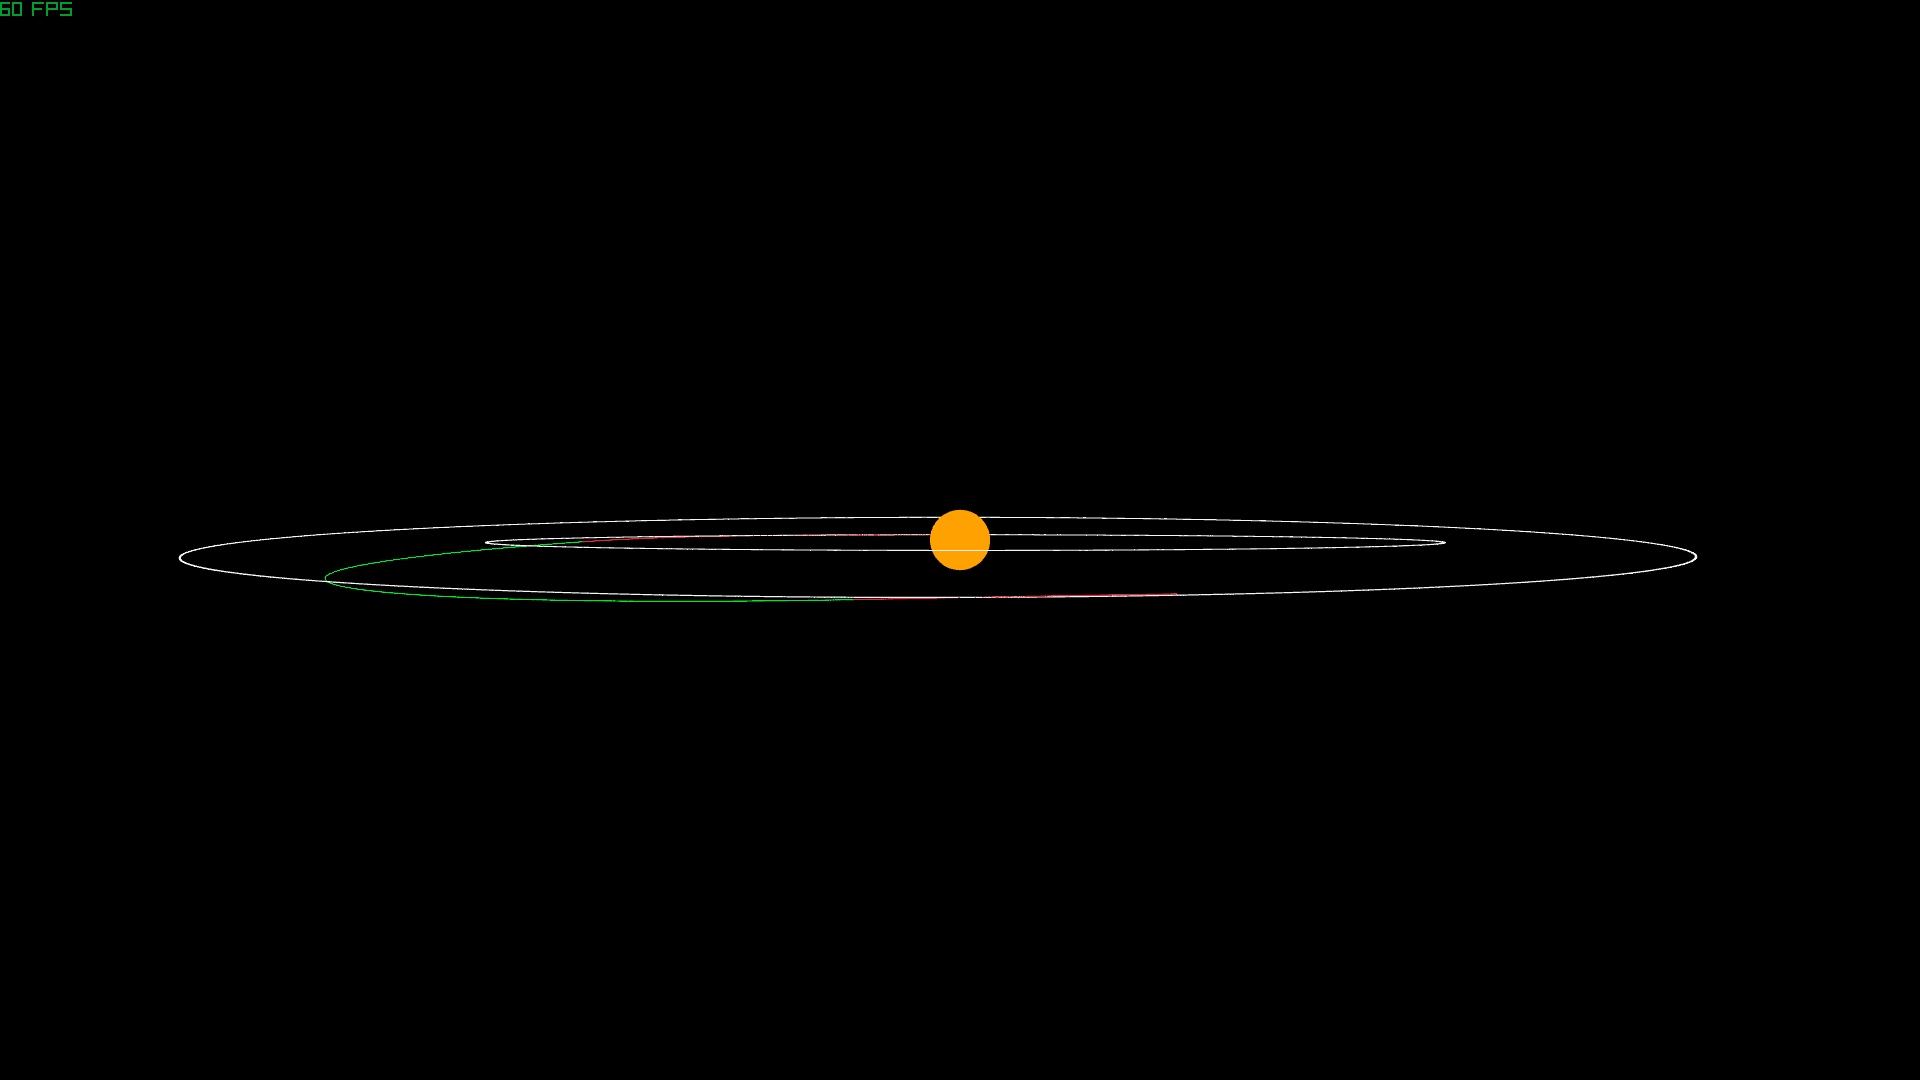
\includegraphics[scale=0.2]{simans4.png}  \\
	\figcaption{模式搜索法优化结果}\label{figSimAns2}
\end{center}


\section{总\quad 结}
本文。


\bibliographystyle{stylebib}
\bibliography{reference}

\end{multicols}
\end{document}
